% typ dokumentu
\documentclass[12pt,twoside]{article}

% użycie pakietu , jak include
\usepackage{weiiszablon}

% autor pracy
\author{Krystian Olszowy}

% np. EF-123456, EN-654321, ..., Numer albumu
\studentID{EA-167582}

\title{Tworzenie drzewa składniowego języka ST}
\titleEN{{Creating an ST language syntax tree}}


%%% wybierz rodzaj pracy wpisując jeden z poniższych numerów: ...
% 1 = inżynierska	% BSc
% 2 = magisterska	% MSc
% 3 = doktorska		% PhD
%%% na miejsce zera w linijce poniżej
\newcommand{\rodzajPracyNo}{2}


%%% promotor
\supervisor{dr inż. Jan Sadolewski}
%% przykład: dr hab. inż. Józef Nowak, prof. PRz

%%% promotor ze stopniami naukowymi po angielsku
\supervisorEN{Jan Sadolewski, PhD, Eng.}


%% DO ZROBIENIA %%
\abstract{Praca zawiera zaproponowane rozwiązanie sterowania telewizorem z poziomu smartfona dzięki aplikacji mobilnej i urządzeniu pośredniczącemu, opartemu o mikrokontroler z niezbędnymi modułami. Przedstawiono i omówiono w niej technologie i koncepty, z których korzystano podczas procesu projektowania i tworzenia rozwiązania. Opisane zostały też najważniejsze elementy fizycznej części systemu, oprogramowanie mikrokontrolera, zbudowana aplikacja mobilna oraz ich współpraca w celu sterowania urządzeniem telewizyjnym.}
\abstractEN{The work encompasses a solution for television control through a smartphone application and an intermediary device, based on a microcontroller with necessary modules. It introduces and discusses the technologies and concepts employed during the design and building process. Additionally, it details the key components of the physical system, microcontroller software, the developed mobile application, and their collaboration for television device control.}

%% DO ZROBIENIA %%
\keywords{ST language, syntax tree, CPDev, ANTLRv4, parser}
\keywordsEN{język ST, drzewo składniowe, CPDev, ANTLRv4, parser}


\begin{document}

% strona tytułowa
\maketitle

\blankpage

% spis treści
\tableofcontents

\clearpage
\blankpage

\section{Wstęp}
\subsection{Zintegrowane środowiska programistyczne (ang. IDE)}
Współczesny inżynier czy programista automatyki nie wyobraża sobie pracy bez dostępu do zintegrowanego środowiska programistycznego (ang. IDE). Środowiska te, będące podstawowym narzędziem w pracy twórców oprogramowania sterowników PLC, przekształciły się z prostych edytorów kodu w zaawansowane platformy wspierające projektowanie, symulację, testowanie i wdrażanie systemów sterowania. Dzięki nim możliwe jest nie tylko wygodne tworzenie logiki sterującej, ale również wizualizacja procesów, zarządzanie konfiguracją sprzętu czy analizowanie działania programu w~czasie rzeczywistym.

Na rynku dostępnych jest wiele rozwiązań, różniących się zakresem funkcji, kompatybilnością z określonymi typami sterowników oraz poziomem zaawansowania użytkownika. Jednym z przykładów takiego środowiska jest CPDev - polskie oprogramowanie tworzone na Politechnice Rzeszowskiej wspierające języki programowania zgodne z normą IEC 61131-3, które umożliwia programowanie sterowników różnych producentów, symulację działania programu oraz jego późniejsze wdrożenie na urządzeniu docelowym. Choć wiele firm korzysta z komercyjnych środowisk oferowanych przez producentów sterowników, takich jak TIA Portal firmy Siemens czy GX Works rozwijane przez Mitsubishi Electronic, to rosnąca popularność rozwiązań niezależnych - jak CPDev - pokazuje, że możliwe jest tworzenie otwartych, elastycznych i konkurencyjnych narzędzi dla branży automatyki.

\subsection{Drzewa składniowe}
Drzewa składniowe to struktury, które trudno przecenić w świecie programowania. Choć na pierwszy rzut oka mogą wydawać się technicznym detalem, w~praktyce są fundamentem działania wielu elementów środowisk programistycznych. To właśnie one przedstawiają kod w uporządkowanej postaci, zgodnej z gramatyką danego języka, dzięki czemu program może być łatwiej analizowany i przetwarzany.

Bez drzew składniowych trudno wyobrazić sobie działanie kompilatorów, interpreterów, a nawet tak podstawowych funkcji edytora jak kolorowanie składni, podpowiadanie składniowe czy automatyczne formatowanie kodu. Dzisiejsze IDE bazują na tych strukturach niemal na każdym kroku - to one pozwalają na bieżąco wykrywać błędy kodu, usprawniają nawigację w projekcie i umożliwiają wprowadzenie inteligentnych podpowiedzi.

Automatyczne generowanie parserów, znacząco przyspiesza proces interpretacji kodu. Dzięki niemu programista nie musi już ręcznie tworzyć złożonych analizatorów składni, co oszczędza czas i~ogranicza liczbę błędów.

Dla środowiska CPDev możliwość generowania drzewa składniowego dla języka ST to istotne ułatwienie. Dzięki temu można nie tylko szybciej i prościej zaimplementować parser zgodny z normą IEC 61131-3, ale też stworzyć solidną podstawę do rozwijania edytora o nowe funkcje - jak choćby inteligentne podpowiedzi, analiza semantyczna czy lepsza diagnostyka błędów. To wszystko przekłada się na wygodniejszą pracę użytkownika i otwiera drogę do dalszego rozwoju CPDeva jako nowoczesnego narzędzia do programowania sterowników.

\subsection{Cel pracy}
Celem pracy jest przygotowanie parsera kodu języka ST zgodnego z normą IEC 61131-3 oraz oprogramowaniem CPDev, generującego drzewo składniowe na~podstawie podanego kodu źródłowego tego języka. Oprogramowanie generujące drzewo składniowe ma współpracować z kodem w języku C\#. Aby takie oprogramowanie przygotować, należy wcześniej także przeprowadzić badanie porównawcze wybranych narzędzi do tworzenia drzew składni języków formalnych opisanych za pomocą gramatyki bezkontekstowej i wybrać rozwiązanie najbardziej odpowiadające postawionemu zadaniu.

\subsection{Zakres pracy}
Zakres pracy obejmuje prównanie wybranych narzędzi do tworzenia drzew skła\-dni języków formalnych opisanych za pomocą gramatyki bezkontekstowej i wybranie najlepszego z nich do analizowania języka ST zgodnego z normą IEC 61131-3 w~CPDevie. Praca podejmuje także tematykę utworzenia pliku gramatyki języka ST dla najbardziej odpowiedniego z analizowanych narzędzi i przetestowania wygenerowanego oprogramowania dla przykładowych kodów źródłowych.


\subsection{Zawartość pracy [DO ZROBIENIA]}
W rozdziale drugim  omówiono ogólnodostępne rozwiązania stanowiące aktualny stan wiedzy w zakresie zdalnego sterowania odbiornikiem telewizyjnym. Prównano je z autorskim systemem wskazując jego zalety i rozwiązywane przez niego problemy.

Rozdział trzeci zawiera przedstawienie i opis technologii wykorzystanych w zaprojektowanym rozwiązaniu. Są to: Platforma ESP32, język programowania C++, framework Arduino, podczerwień, system Android, język programowania Dart, framework Flutter oraz techonlogia Bluetooth Low Energy.

Czwarty rozdział opisuje sposób połączenia komponentów składających się na urządzenie pośredniczące zbudowane aby skomunikować aplikację mobilną z telewizorem. Zawarte zostały w nim także opisane scharakteryzowane parametry tych komponentów.

W rozdziale piątym szczegółowo omówiono utworzone oprogramowanie mikrokontrolera odpowiedzialne za sterowanie jego zasobami i dołączonymi modułami fizycznymi. Przedstawione zostały ważniejsze kody źródłowe projektu oraz ich działanie.

Rozdział szósty zawiera opis zaprojektowanego intefejsu użytkownika aplikacji mobilnej oraz jej funkcjonalności. Ukazane zostały także wykorzystane podczas implementacji, rozwiązania programowe.

Siódmy rozdział koncentruje się na przedstawieniu sposobu korzystania z utworzonego rozwiązania. Dokonywana jest także ocena skuteczności działania poszczególnych funkcji systemu.

W ostatnim rozdziale zawarto podsumowanie całej pracy, możliwe usprawnienia zaprojektowanego rozwiązania. Wskazane zostały też elementy projektu, które autor uważa za wkład własny.


\clearpage
\section{Środowisko CPDev}
\subsection{Charakterystyka narzędzia}
CPDev (Control Program Developer) to otwarte, uniwersalne środowisko inżynierskie przeznaczone do tworzenia i wdrażania oprogramowania sterującego dla systemów automatyki. Powstało jako efekt wieloletnich prac badawczych i rozwojowych prowadzonych na Politechnice Rzeszowskiej. Głównym założeniem projektowym CPDev było stworzenie platformy, która będzie nie tylko zgodna z normą IEC 61131-3, ale również łatwa do przeniesienia na różne platformy sprzętowe i dostępna dla inżynierów oraz studentów jako narzędzie zarówno edukacyjne, jak i przemysłowe\cite{cpdevKia}.

Jednym z głównych atutów CPDev jest modularność oraz szeroki zakres funkcjonalności obejmujący cały proces tworzenia aplikacji sterujących. Środowisko udostępnia zestaw edytorów tekstowych i graficznych, narzędzia do konfiguracji systemu, symulator sterownika oraz narzędzia do projektowania interfejsów HMI. Dzięki temu możliwe jest kompleksowe projektowanie i testowanie systemów sterowania bez konieczności stosowania zewnętrznych narzędzi.

Ważną cechą CPDev-a jest jego niezależność sprzętowa, osiągnięta dzięki zastosowaniu warstwy pośredniej w postaci maszyny wirtualnej, która interpretuje kod pośredni generowany przez kompilator. Takie podejście umożliwia łatwe wdrażanie systemu na różnych urządzeniach, w tym na mikrokontrolerach, procesorach ARM, a nawet na implementacjach FPGA\cite{cpdevFPGA}. Jednocześnie zapewnia ono jednolity sposób działania aplikacji niezależnie od platformy sprzętowej.

Środowisko CPDev jest stale rozwijane i udoskonalane. W kolejnych wersjach wprowadzano m.in. wsparcie dla języków graficznych, rozszerzenia dla systemów wielordzeniowych, interfejsy XML pozwalające na współpracę z innymi narzędziami inżynierskimi oraz rozwiązania umożliwiające projektowanie zgodnie z podejściem MDD (Model-Driven Development). CPDev znalazł już zastosowanie w wielu wdrożeniach przemysłowych — zarówno w kraju, jak i za granicą.

Z punktu widzenia użytkownika, środowisko CPDev oferuje funkcjonalności znane z komercyjnych rozwiązań, przy czym wyróżnia się większą otwartością, możliwością adaptacji do konkretnych potrzeb oraz dostępnością szczegółów implementacyjnych. To wszystko sprawia, że CPDev stanowi atrakcyjną alternatywę wobec zamkniętych środowisk oferowanych przez producentów sprzętu automatyki.
\subsection{Programowanie za pomocą CPDev-a}
\subsubsection{Ogólny sposób korzystania z narzędzia}
Programowanie w środowisku CPDev odbywa się w ramach graficznego interfejsu IDE, które integruje różne etapy projektowania systemu automatyki: od pisania kodu sterującego, przez konfigurację sprzętu i symulację, aż po wdrożenie na urządzenie docelowe \cite{cpdev2009}. Proces ten można podzielić na kilka etapów:

\begin{enumerate}[label=\arabic*), leftmargin=1.25cm]
    \item Tworzenie projektu -- użytkownik definiuje strukturę programu, dodaje nowe jednostki organizacyjne (POUs), deklaruje zmienne globalne i lokalne.
    \item Kodowanie logiki sterowania -- za pomocą jednego lub kilku języków normy IEC 61131-3.
    \item Konfigurację sprzętu i zmiennych wejścia-wyjścia -- z użyciem narzędzia CPCon.
    \item Symulację i testowanie -- możliwą dzięki narzędziu CPSim, które pozwala uruchomić aplikację sterującą w trybie offline.
    \item Generowanie kodu pośredniego (VMASM) -- po kompilacji, aplikacja może zostać załadowana do wirtualnej maszyny uruchamianej na docelowym sterowniku.
\end{enumerate}

\subsubsection{Dostępne języki programowania sterowników}
CPDev wspiera wszystkie języki określone w normie IEC 61131-3\cite{iec61131-3}\cite{cpdevLanguages}, co pozwala użytkownikom wybrać najbardziej pasujący im sposób definiowania logiki sterującej w zależności od specyfiki projektu lub preferencji osobistych. Szczegółowo, obsługiwane przez CPDev języki programowania to:

\begin{enumerate}[label=\alph*), leftmargin=1.25cm]
    \item ST (Structured Text)\\
    Język ST jest tekstowym językiem wysokiego poziomu, przypominającym składnią Pascal i języki z rodziny C. Oferuje bogaty zestaw struktur sterujących (pętle, warunki itp.), obsługę typów prostych i złożonych (strukturalnych i obiektowych) oraz wyrażeń logicznych i arytmetycznych. CPDev umożliwia pisanie całych aplikacji w ST, a także używanie go do definiowania funkcji i bloków funkcyjnych. Edytor kodu ST w CPDev jest wyposażony w podświetlanie składni, autouzupełnianie i sprawdzanie błędów składniowych na bieżąco, co znacznie ułatwia pracę programisty. Okno edycji z przykładowym kodem ST przedstawiono na rysunku \ref{Fig:startStopST}.

   \begin{figure}[ht]
   \centering
   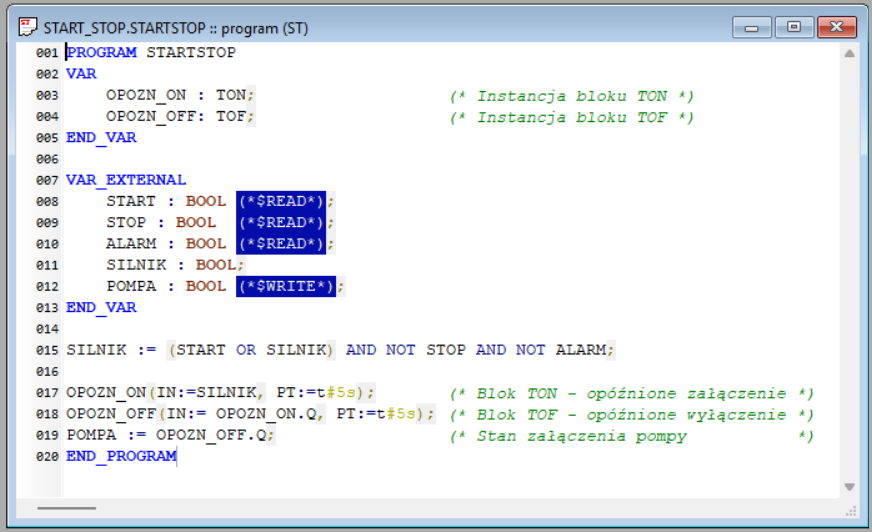
\includegraphics[width=12cm]{images/startStopST.png}
   \caption{Okno edycji prostego kodu ST w programie CPDev}
   \label{Fig:startStopST}
   \end{figure}

    \item IL (Instruction List)\\
    IL to język niskopoziomowy, przypominający assembler. Umożliwia precyzyjne określanie instrukcji operujących na rejestrach i zmiennych. Jego stosowanie w CPDev jest obecnie rzadsze, ponieważ został wycofany z najnowszej wersji normy IEC 61131-3, ale nadal pozostaje dostępny dla kompatybilności. Okno edycji IL w CPDev pozwala na pisanie kodu w formie instrukcji, przedstawiono je wraz z przykładowym kodem na rysunku \ref{Fig:startStopIL}. 

   \begin{figure}[ht]
   \centering
   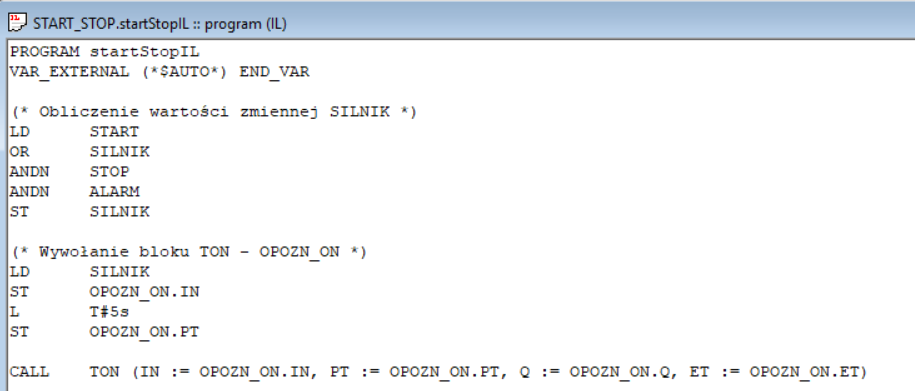
\includegraphics[width=13cm]{images/startStopIL.png}
   \caption{Okno edycji prostego kodu IL w programie CPDev}
   \label{Fig:startStopIL}
   \end{figure}

    \item FBD (Function Block Diagram)\\
    FBD jest językiem graficznym, który pozwala na tworzenie logiki poprzez łączenie bloków funkcjonalnych w sposób przypominający schematy blokowe. Jest chętnie wykorzystywany przez inżynierów o mniejszym doświadczeniu programistycznym, szczególnie w przemyśle. W CPDev edytor FBD umożliwia tworzenie diagramów blokowych, gdzie każdy blok reprezentuje funkcję lub operację, a~połączenia między nimi definiują przepływ danych. Bloki mogą być konfigurowane i łączone w sposób graficzny, co ułatwia zrozumienie logiki sterowania. Przykładowe okno edycji FBD z prostym kodem przedstawiono na rysunku \ref{Fig:startStopFBD}.

   \begin{figure}[ht]
   \centering
   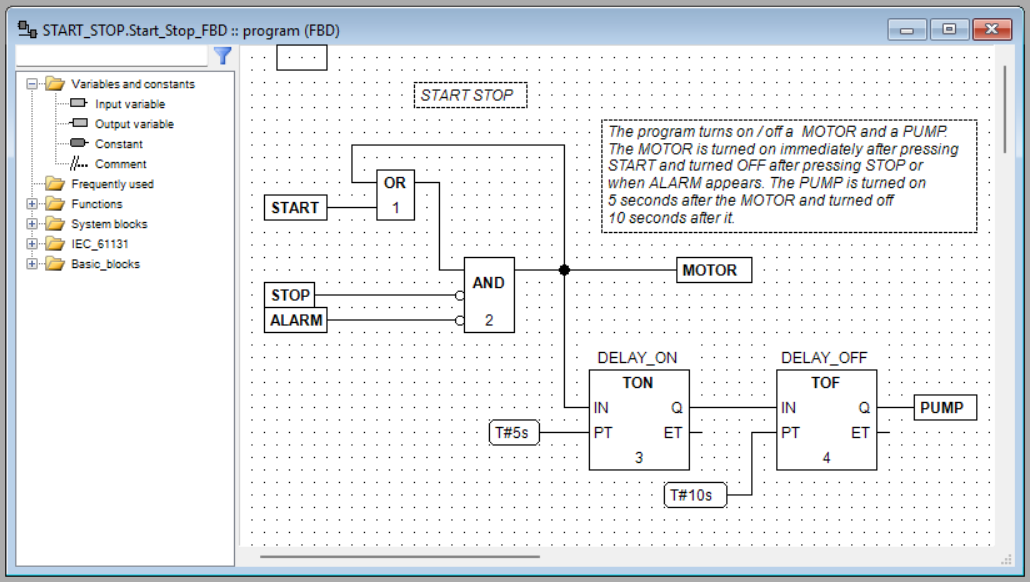
\includegraphics[width=14cm]{images/startStopFBD.png}
   \caption{Okno edycji prostego kodu FBD w programie CPDev}
   \label{Fig:startStopFBD}
   \end{figure}

    \item LD (Ladder Diagram)\\
    LD, znany także jako język drabinkowy, to język graficzny inspirowany schematami przekaźnikowymi. Ułatwia migrację klasycznych systemów sterowania przekaźnikowego do programowalnych sterowników PLC. CPDev umożliwia tworzenie programów w LD i konwersję do ST. Edytor LD pozwala na graficzne definiowanie logiki sterującej w formie drabinki, gdzie symbole reprezentują elementy logiczne (przekaźniki, styki, cewki), a połączenia między nimi definiują przepływ sygnałów. Przykładowe okno edycji LD z prostym kodem przedstawiono na rysunku \ref{Fig:startStopLD}.

   \begin{figure}[ht]
   \centering
   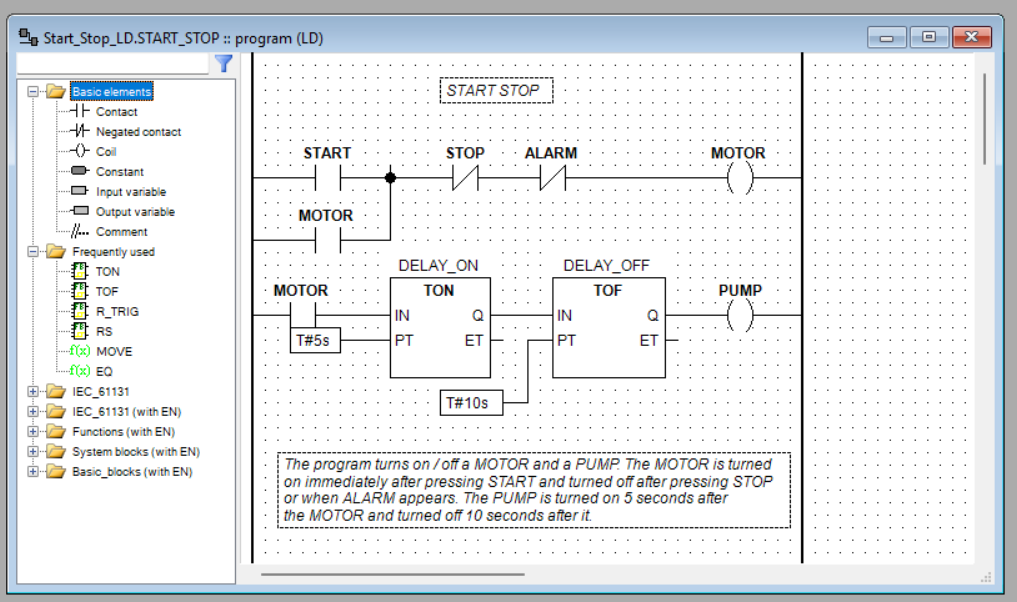
\includegraphics[width=12cm]{images/startStopLD.png}
   \caption{Okno edycji prostego kodu LD w programie CPDev}
   \label{Fig:startStopLD}
   \end{figure}

    \item SFC (Sequential Function Chart)\\
    SFC jest językiem służącym do modelowania logiki sekwencyjnej. Program składa się z kroków, przejść i warunków przejścia. W CPDev sekwencyjna struktura tworzona jest graficznie, a logika kroków i przejść może być zapisana w ST lub FBD. Edytor SFC w CPDev pozwala na tworzenie diagramów sekwencyjnych, gdzie każdy krok reprezentuje stan systemu, a przejścia między nimi definiują warunki przejścia. Przykładowe okno edycji SFC z prostym kodem przedstawiono na rysunku \ref{Fig:tanksSFC}.

   \begin{figure}[ht]
   \centering
   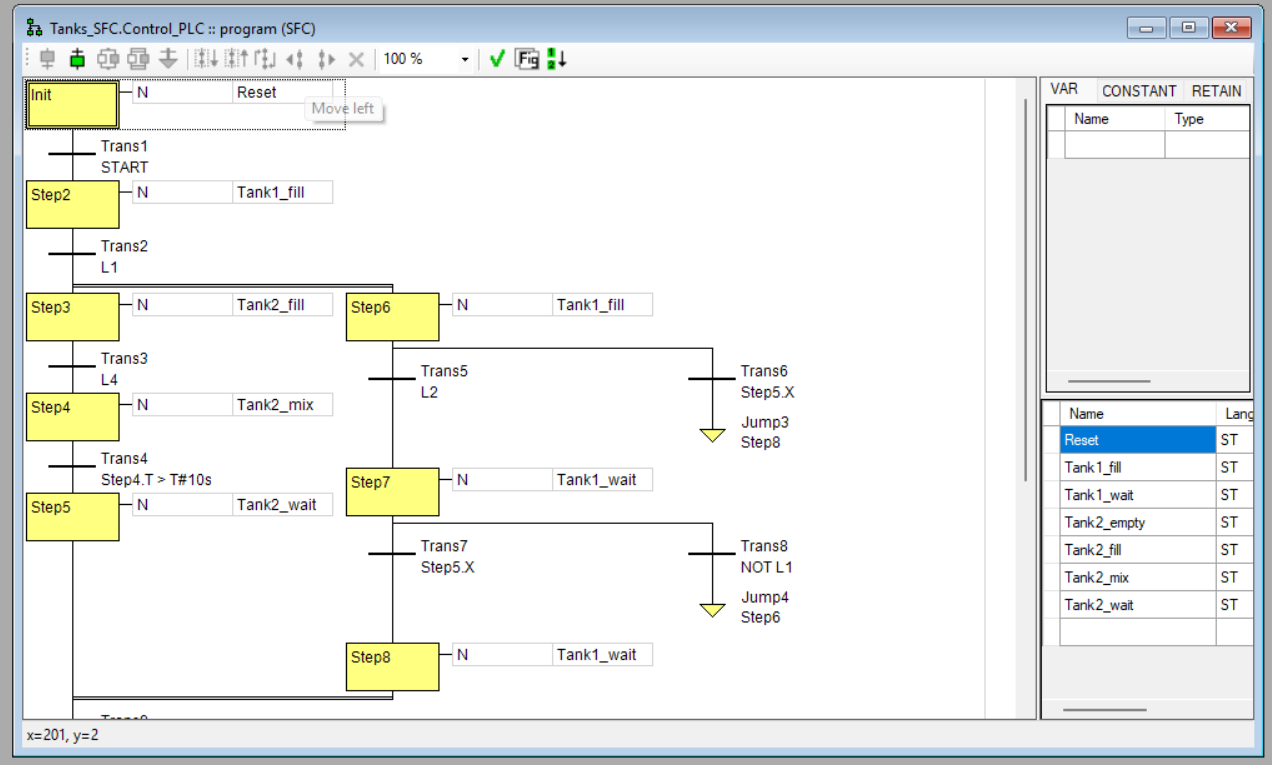
\includegraphics[width=12cm]{images/tanksSFC.png}
   \caption{Okno edycji prostego kodu SFC w programie CPDev}
   \label{Fig:tanksSFC}
   \end{figure}
\end{enumerate}

\subsection{Implementacja CPDev-a i architektura maszyny wirtualnej}

Implementacja środowiska CPDev została oparta na założeniu, że system sterowania powinien być niezależny od konkretnej platformy sprzętowej, a zarazem możliwy do wdrożenia w rzeczywistych aplikacjach przemysłowych. Aby to osiągnąć, architektura CPDev została podzielona na dwa główne poziomy: środowisko deweloperskie (IDE) oraz maszynę wirtualną (VM), która wykonuje wygenerowany program sterujący.

Środowisko deweloperskie CPDev zostało zaimplementowane w języku C\# na platformę .NET, przez co aplikacja posiada nowoczesny interfejs graficzny, zapewnia wygodę użytkowania i łatwość dalszej rozbudowy. Składa się z modularnych komponentów, takich jak edytory kodu źródłowego, narzędzia konfiguracyjne, symulatory, analizatory błędów i generator kodu pośredniego \cite{cpdevOverview}. Zastosowanie C\# i środowiska .NET pozwala na integrację z innymi narzędziami, obsługę graficznych języków programowania oraz wprowadzanie rozwiązań typowych dla nowoczesnych aplikacji okienkowych (GUI).

Jednym z najważniejszych elementów tego środowiska jest kompilator, który tłumaczy kod źródłowy napisany w językach normy IEC 61131-3 (głównie ST, gdyż inne języki są na niego tłumaczone) do VMASM, czyli pośredniego kodu niskiego poziomu wykonywanego przez maszynę wirtualną. Maszyna wirtualna CPDev-a to lekki, niezależny od sprzętu interpreter kodu VMASM, implementowany głównie w języku ANSI C, co zapewnia wysoką przenośność. Dzięki temu może ona działać na wielu różnych platformach sprzętowych, w tym na mikrokontrolerach (np. AVR, ARM), systemach wbudowanych (np. Raspberry Pi, STM32), a także w symulacji na komputerze PC\cite{cpdevVM}.

\begin{figure}[ht]
   \centering
   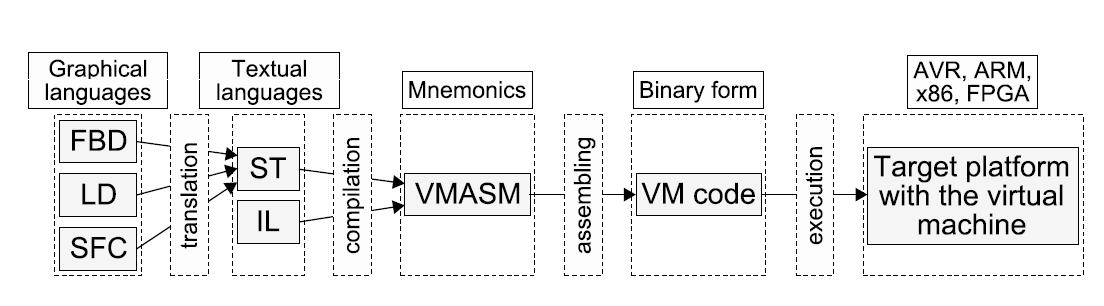
\includegraphics[width=15cm]{images/cpdevScheme.png}
   \caption{Schemat przetwarzania kodu użytkownika w środowisku CPDev\cite{cpdevOperations}}
   \label{Fig:cpdevScheme}
\end{figure}

\clearpage

\section{Drzewa składniowe na podstawie gramatyk bezkontekstowych}
\subsection{Wprowadzenie do gramatyk bezkontekstowych}
Gramatyki bezkontekstowe (CFG, Context-Free Grammar) to matematyczny model służący do opisu struktury formalnych języków, takich jak języki programowania. Składają się one z:
\begin{itemize}[label=\textbullet, leftmargin=1.25cm]
   \item skończonego zbioru symboli nieterminalnych (zmiennych),
   \item zbioru symboli terminalnych (symboli końcowych, np. słów kluczowych, operatorów),
   \item zestawu produkcyjnych reguł, w których każdy symbol nieteminalny może być zastąpiony ciągiem terminali oraz nieterminali, 
   \item specjalnego symbolu startowego.
\end{itemize} 
Najważniejszą ich cechą jest to, że zachowują swoje znaczenie niezależnie od kontekstu czyli otoczenia, w którym znajduje się symbol. Gramatyki bezkontekstowe są wystarczająco złożone, by opisać większość języków programowania, ale jednocześnie na tyle proste, by dawać się wydajnie parsować algorytmicznie.\cite{contextFreeGrammar}

\subsection{Wyprowadzenia i formy zdaniowe}
Proces generowania ciągu terminali rozpoczyna się od symbolu startowego i~polega na wielokrotnym zastępowaniu nieterminali zgodnie z regułami gramatyki rozwijając kolejno każdy symbol nieterminalny\cite{contextFreeGrammar}. Taki proces to wyprowadzanie, często opisywany za pomocą kroków typu lewostronnego lub prawostronnego. W każdym etapie generowania terminali powstają tzw. formy zdaniowe, czyli częściowo przetworzone ciągi symboli.

\subsection{Drzewa składniowe}
Drzewo składniowe to uporządkowana struktura w postaci drzewa, która wizualnie i strukturalnie odwzorowuje sposób, w jaki ciąg symboli terminalnych (np. kod programu) został wygenerowany przez gramatykę. Korzeń drzewa to symbol startowy, a każdy węzeł wewnętrzny reprezentuje symbol nieterminalny, który został rozwinięty na swoje dzieci (symbole terminalne lub inne nieterminale). Z kolei liście drzewa odpowiadają symbolom terminalnym, które są końcowymi elementami wygenerowanego ciągu.

Drzewo składniowe powstaje podczas procesu parsowania kodu: każda reguła produkcyjna zamienia symbol nieterminalny na jego dzieci w~drzewie. Korzystając z~kolejności liści od lewej lub prawej, odczytać można oryginalny ciąg słów, czyli w~przypadku zastosowania dla CPDev: kod źródłowy. Poniżej na rysunku \ref{Fig:simpleGrammarTree} przedstawiono przykład drzewa składniowego dla prostego wyrażenia arytmetycznego \textit{7 + 2 * 3} z~zastosowaniem zasad znanych z~matematyki, gdzie mnożenie ma wyższy priorytet niż dodawanie.

\begin{figure}[ht]
   \centering
   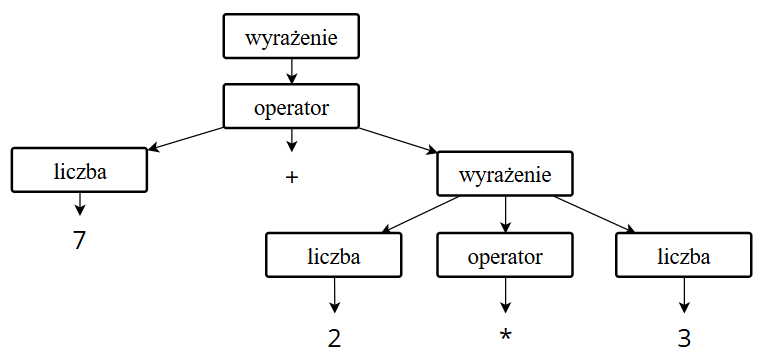
\includegraphics[width=15cm]{images/grammarTreeSimple.png}
   \caption{Drzewo składniowe dla prostego wyrażenia arytemtycznego \textit{7 + 2 * 3}}
   \label{Fig:simpleGrammarTree}
\end{figure}

Drzewa składniowe mogą służyć jako:
\begin{itemize}[label=\textbullet, leftmargin=1.25cm]
   \item reprezentacja struktury kodu źródłowego, na przejrzystym diagramie pokazującym hierarchię i zależności między elementami,
   \item podstawa do analiz semantycznych, takich jak sprawdzanie typów czy wykrywanie błędów,
   \item model na którego podstawie zostanie wygerenowany kod pośredni lub docelowy wykorzystywany w kompilatorach i interpreterach.\\\\
\end{itemize}

\subsection{Zastosowanie parserów w IDE}
W zintegrowanych środowiskach programistycznych drzewa składniowe są podstawą kolorowania składni, dynamicznych podpowiedzi, sprawdzanie błędów składniowych, a także automatycznej refaktoryzacji kodu. Dla CPDev-a z uwagi na to, że korzysta on z translatora kodu źródłowego, drzewo składniowe kodu języka ST jest niezbędne do poprawnej analizy i interpretacji kodu. Automatyczna generacja drzewa składniowego na podstawie pliku gramatyki pozwoliłaby na ujednolicenie procesu tworzenia parsera, co jest niezwykle istotne dla rozwoju środowiska CPDev. Dzięki temu możliwe byłoby łatwiejsze wprowadzanie zmian w gramatyce języka ST oraz szybsze dostosowywanie parsera do nowych wymagań.
\clearpage

\section{Przegląd narzędzi do tworzenia parserów automatycznie generujących drzewa składniowe}

W niniejszej pracy parser składniowy posłuży do analizy utworzenia drzewa składniowego języka Structured Text (ST), który jest jednym z pięciu języków programowania określonych w normie IEC 61131-3, używanych do programowania sterowników PLC. Parser ten zostanie zastosowany w ramach oprogramowania CPDev. Celem jest wygenerowanie drzewa składniowego programu ST, które może zostać następnie wykorzystane do dalszych analiz semantycznych, optymalizacji lub transformacji kodu źródłowego.

Z uwagi na specyfikę CPDev-a utworzonego w języku C\# i bazującego na strukturach .NET istotne jest, aby wybrane narzędzie do generowania parserów było kompatybilne z tą platformą, a także zapewniało czytelność, rozszerzalność i dobrą integrację z pozostałymi komponentami systemu. W dalszej części tego rozdziału przeprowadzona zostanie analiza wybranych narzędzi do tworzenia parserów automatycznie generujących drzewa składniowe pod kątem ich funkcjonalności, wydajności, wsparcia dla języka C\# oraz możliwości integracji z systemem CPDev. Na tej podstawie zostanie dokonany wybór najlepszego rozwiązania.
\subsection{ANTLRv4}

ANTLR (ANother Tool for Language Recognition) to generator parserów opracowany przez Terence'a Parra i jego zespół. Jego najnowsza wersja czyli ANTLRv4 została wydana w sierpniu 2024 roku i jest objęta licencją BSD3. Narzędzie to stanowi kulminację ponad 25 lat badań nad technikami parsowania języków formalnych. 

ANTLRv4 wpiera aż 10 jezyków docelowych\cite{antlr4GitHub}, w których może zostać utworzony parser i są to: C++, C\#, Dart, Java, JavaScript, PHP, Python3, Swift, TypeScript oraz Go. Wykorzystywany jest w projektach akademickich i przemysłowych takich jak m.in. Twitter (zapytania), Hive i Pig w Hadoop, narzędzia Oracle (SQL Developer), Hibernate, NetBeans, Presto czy MySQL Workbench.\cite{antlr4Org}

\subsubsection{Typ gramatyki i parsera}
ANTLRv4 w utworzonym parserze wykorzystuje algorytm Adaptive LL(*), często skracany jako ALL(*), będący znaczącym ulepszeniem względem klasycznych parserów LL(k) i wcześniejszej wersji ANTLRv3. W przeciwieństwie do statycznego LL(), ALL() dokonuje analizy lookahead dynamicznie podczas działania parsera, co pozwala na obsłużenie bardziej złożonych oraz naturalnych gramatyk bez konieczności ręcznej transformacji reguł.\cite{antlr4GitHub} Eliminuje też konieczność backtrackingu, typową dla wcześniejszych wersji ANTLR w sytuacjach niejednoznacznych\cite{Antlr4Optimisation}. Poniżej na listingu \ref{Lst:antlrv4SimpleGrammar} przedstawiono przykładową prostą gramatykę dla ANTLRv4 gdzie można zauważyć, że nie było wymagane wykonywanie skomplikowanej struktury zagnieżdżonej znanej z~parserów typu top-down\cite{antlr4Book}, którym w istocie jest parser generowany przez to narzędzie.

\lstinputlisting[inputencoding=utf8/cp1250, language={bash}, caption={\protect\input{captions/antlrv4SimpleGrammar.txt}\protect\relax}, label={Lst:antlrv4SimpleGrammar}]{codes/antlrv4SimpleGrammar.txt}

ANTLRv4 umożliwia definiowanie reguł z rekurencją lewą np. \kod{expr: expr '+' expr;} co wcześniej było niemożliwe i sprawiało trudności w parserach typu top-down. Reguły te są automatycznie przekształcane przez ANTLR na odpowiedniki bez rekurencji przez wbudowane mechanizmy przepisujące gramatykę, zachowując przy tym prawidłową kolejność operatorów i skojarzenia. Jednak ANTLR obsługuje wyłącznie bezpośrednią rekurencję lewą i nie wspiera rekurencji pośredniej (czyli wzajemnej między różnymi regułami parsera).

\subsubsection{Ogólny proces generowania parsera}
Proces tworzenia parsera za pomocą ANTLRv4 składa się z kilku nieskomplikowanych dla użytkownika kroków, które umożliwiają automatyczne wygenerowanie analizatora składniowego na podstawie formalnej gramatyki języka:

\begin{enumerate}[label=\arabic*., leftmargin=1.25cm]
\item 
Zdefiniowanie gramatyki -- Pierwszym krokiem jest utworzenie pliku z rozszerzeniem \kod{.g4}, w którym zapisuje się reguły gramatyki w notacji zbliżonej do EBNF. Gramatyka zawiera definicje tokenów (reguły leksykalne) oraz struktur językowych (reguły parsera).
\item Uruchomienie generatora -- Korzystając z narzędzia antlr4 (np. z wiersza poleceń), generuje się zestaw klas parsera i leksera w wybranym języku programowania (np. C\#, Java, Python). Na przykład dla języka C\#:\\
 \kod{java -jar antlr-4.X-complete.jar -Dlanguage=CSharp Expr.g4}
\item Integracja z aplikacją -- Wygenerowane klasy mogą zostać dołączone do projektu w wybranym środowisku programistycznym. Z parsera można korzystać poprzez utworzenie instancji klasy leksera i parsera, a następnie przekazanie do nich kodu źródłowego jako tekstu.
\item Obsługa wynikowego drzewa składniowego -- ANTLR umożliwia automatyczne przetwarzanie wygenerowanego drzewa składniowego przy pomocy wzorców Visitor lub Listener.
\item Obsługa błędów i debugowanie -- Parser domyślnie obsługuje wykrywanie i raportowanie błędów składniowych, a dodatkowo użytkownik może nadpisać domyślne zachowanie narzędzia w przypadku wykrycia błędu(np. logowanie, zatrzymanie parsowania lub odzyskiwanie po błędach).
\end{enumerate}

Dzięki oddzieleniu gramatyki od logiki aplikacji i wsparciu wielu języków programowania, ANTLRv4 umożliwia łatwe i szybkie tworzenie parserów z pełnym drzewem składniowym gotowym do dalszego przetwarzania.

\subsubsection{Tworzenie gramatyki}
Gramatyka w ANTLR v4 zapisywana jest w plikach z rozszerzeniem \kod{.g4} i definiowana w notacji zbliżonej do EBNF (Extended Backus-Naur Form). Plik gramatyki zawiera dwie główne sekcje:
\begin{itemize}[label=\textbullet, leftmargin=1.25cm]
   \item Reguły parsera -- definiują strukturę języka, czyli jak poszczególne elementy (np. wyrażenia, instrukcje) są zbudowane z tokenów. Nazwy reguł zaczynają się małą literą.
   \item Reguły leksykalne -- definiują tokeny, czyli podstawowe elementy składniowe (np. liczby, słowa kluczowe, operatory). Nazwy reguł zaczynają się wielką literą.
\end{itemize}
Aby zobrazować sposób tworzenia gramatyki w ANTLR v4, poniżej na listingu  \ref{Lst:antlrv4BiggerGrammar}  przedstawiono prostą gramatykę dla wyrażeń arytmetycznych i przypisań. Na początku definiowana jest w niej reguła startowa \kod{program}, która określa, że analizowany tekst składa się z wielu instrukcji zakończonych końcem pliku. Następnie wprowadzone są reguły odpowiadające różnym typom instrukcji, takim jak przypisania i instrukcje warunkowe. Dalej znajduje się reguła \kod{expr}, która opisuje strukturę wyrażeń arytmetycznych i odniesień do zmiennych.

W drugiej części gramatyki znajdują się reguły leksykalne. Określają one sposób rozpoznawania słów kluczowych, identyfikatorów i liczb całkowitych. Na końcu dodano reguły pomijające znaki białe oraz komentarze, aby nie były uwzględniane w analizie składniowej.

\lstinputlisting[inputencoding=utf8/cp1250, language={bash}, caption={\protect\input{captions/antlrv4BiggerGrammar.txt}\protect\relax}, label={Lst:antlrv4BiggerGrammar}]{codes/antlrv4BiggerGrammar.txt}

\subsubsection{Analiza drzewa składniowego}
ANTLRv4 automatycznie generuje pełne drzewo składniowe (Concrete Syntax Tree, CST) na podstawie zdefiniowanej gramatyki. Drzewo to reprezentuje dokładną strukturę analizowanego kodu źródłowego i może być wykorzystane do dalszego przetwarzania na różne sposoby. Na grafice poniżej przedstawiono przykładowe drzewo składniowe wygenerowane przez ANTLRv4 dla prostego kodu ST, który przypisuje wartość do zmiennej i wykonuje operację arytmetyczną, a także korzysta w wyrażenia warunkowego. Widać w nim strukturę hierarchiczną, gdzie każdy węzeł reprezentuje regułę gramatyczną lub token.

\begin{figure}[ht]
   \centering
   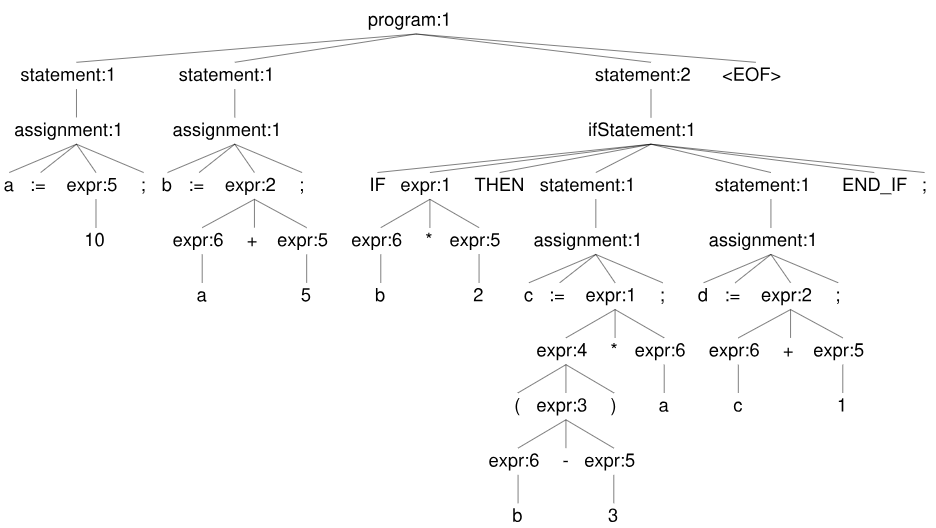
\includegraphics[width=15cm]{images/biggerTreeSimple.png}
   \caption{Drzewo składniowe dla prostego kod ST wcześniej opisanej prostej gramatyki}
   \label{Fig:biggerGrammarTree}
\end{figure}

Jednym z najczęściej stosowanych podejść jest wzorzec \kod{Visitor}, który pozwala na kontrolowane przechodzenie po węzłach drzewa i wykonywanie operacji zależnych od typu konstrukcji składniowej. Wzorzec ten doskonale sprawdza się przy analizie semantycznej, generowaniu kodu lub przekształceniach drzewa. Alternatywnie, ANTLR udostępnia również mechanizm \kod{Listenera}, który umożliwia reagowanie na wejście i~wyjście z każdego węzła reguły gramatycznej w kolejności predefiniowanej przez parser. Listener sprawdza się m.in. przy prostym zbieraniu informacji lub pasywnym śledzeniu struktury kodu.

W praktyce często zachodzi potrzeba uproszczenia struktury drzewa składniowego poprzez konwersję CST do własnej reprezentacji AST (Abstract Syntax Tree). ANTLR nie robi tego automatycznie, ale umożliwia łatwe ręczne budowanie AST podczas odwiedzania węzłów drzewa — np. przez klasy Visitor.

Dodatkowo ANTLR wspiera narzędzia wizualne, takie jak ANTLR Tool czy ANTLRWorks, które pozwalają graficznie przeglądać drzewa składniowe i śledzić przebieg analizy. Ułatwia to zarówno testowanie parsera, jak i debugowanie trudnych przypadków związanych z niejednoznacznością lub błędami składniowymi.

\subsubsection{Obsługa błędów}
ANTLR udostępnia zaawansowane mechanizmy obsługi błędów składniowych, które umożliwiają zarówno wykrywanie, jak i kontrolowane reagowanie na nieprawidłowości w analizowanym kodzie źródłowym. Domyślnie parser korzysta z klasy \kod{DefaultErrorStrategy}, która implementuje mechanizm tzw. odzyskiwania po błędach. Zamiast przerywać analizę po wykryciu pierwszego błędu, parser stara się kontynuować analizę wejścia, ignorując fragmenty niezgodne z gramatyką lub dokonując prostych poprawek (np. pominięcie niespodziewanego tokena lub podstawienie brakującego). Takie podejście pozwala parserowi wykryć i zgłosić wiele błędów w jednym przebiegu, co jest szczególnie przydatne przy analizie większych plików źródłowych, których czas analizy zaczyna być znaczący.

W sytuacjach, w których wymagana jest ścisła zgodność z gramatyką, można zastosować strategię \kod{BailErrorStrategy}, która natychmiast przerywa analizę po napotkaniu pierwszego błędu składniowego. Taki sposób działania znajduje zastosowanie w przypadkach, gdzie analiza częściowo niepoprawnego kodu nie ma sensu lub gdy parser ma być elementem wrażliwego systemu przetwarzania danych, gdzie konieczna jest pełna poprawność wejścia.

ANTLR pozwala na implementację własnych strategii obsługi błędów, poprzez dziedziczenie po klasie \kod{ANTLRErrorStrategy} lub \kod{BaseErrorListener}. Dzięki temu możliwe jest dokładne dostosowanie sposobu raportowania błędów do potrzeb projektu przez na przykład wzbogacenie komunikatów diagnostycznych, przekazywanie błędów do logów systemowych, a także kontrola lokalizacji i kontekstu błędów. 

ANTLRv4 umożliwia również podłączenie wielu klas nasłuchujących na błędy (ang. error listeners), co pozwala na jednoczesne rejestrowanie informacji o błędach w różnych miejscach jak na przykład zapisywanie ich do pliku, wyświetlanie komunikatów w interfejsie graficznym aplikacji czy gromadzenie szczegółowych danych diagnostycznych na potrzeby testów automatycznych. Programista przez to otrzymuje dużą elastyczność w zarządzaniu błędami i może dostosować sposób ich obsługi do specyfiki projektu oraz potrzeb użytkowników końcowych.\cite{antlr4Book}

Zaawansowana obsługa błędów to jedna z największych zalet ANTLRv4. Parser może być skonfigurowany zarówno do pracy w trybie diagnostycznym, gdzie szczegółowo raportuje i analizuje wszystkie napotkane nieprawidłowości, jak i w trybie produkcyjnym, gdzie nacisk kładziony jest na stabilność działania i szybkie informowanie użytkownika o problemach. Dzięki temu ANTLR sprawdza się w praktycznych zastosowaniach, w których istotne jest nie tylko poprawne przetwarzanie poprawnego kodu, ale również skuteczne wykrywanie i obsługa błędów popełnianych przez użytkowników. Pozwala to na budowanie bardziej przyjaznych i odpornych na błędy narzędzi programistycznych, które lepiej wspierają proces tworzenia oprogramowania.
\subsubsection{Wydajność i rozszerzalność}
ANTLRv4 wykorzystuje strategię parsowania LL(*), która umożliwia analizę składniową z dowolnie długim spojrzeniem w przód. W praktyce parsery generowane przez to narzędzie zapewniają wydajność wystarczającą do większości zastosowań, zwłaszcza w przypadku języków o umiarkowanej złożoności, takich jak ST. Warto jednak zauważyć, że w przypadku bardzo dużych lub silnie niejednoznacznych gramatyk, parsery LL(*) mogą działać wolniej niż analizatory oparte na technikach LR (np. LALR czy GLR).\cite{antlr4Performance} Wybór odpowiedniego narzędzia powinien być więc uzależniony od specyfiki projektu i wymagań dotyczących wydajności.

ANTLR umożliwia rozbudowę parserów o własne akcje semantyczne, klasy pomocnicze czy dodatkowe mechanizmy przetwarzania. Pozwala to na dostosowanie działania parsera do konkretnych potrzeb, na przykład poprzez implementację własnych systemów diagnostycznych lub logujących. Narzędzie wspiera także modularne projektowanie analizatorów, co ułatwia rozwijanie poszczególnych elementów, takich jak lexer, parser czy AST visitor, w sposób niezależny. Dzięki temu parsery generowane przez ANTLR mogą być wykorzystywane zarówno w prostych projektach, jak i w bardziej złożonych systemach, gdzie wymagane jest dalsze przetwarzanie drzewa składniowego, analiza semantyczna czy generowanie kodu.

\subsubsection{Dokumentacja, licencja i wsparcie społeczności}
ANTLR v4 jest bardzo dobrze udokumentowanym i aktywnie rozwijanym narzędziem, przez co jest przyjaznym wyborem zarówno dla początkujących, jak i zaawansowanych użytkowników. Podstawowym źródłem wiedzy jest oficjalne repozytorium, które zawiera dokumentację, przykłady oraz zestaw narzędzi i pluginów wspierających różne języki programowania. Dodatkowo, autor narzędzia Terence Parr opracował obszerną książkę ,,The Definitive ANTLR 4 Reference'', która w przystępny sposób omawia zasady działania parsera, projektowania gramatyk i integracji z kodem użytkownika.

Dużym atutem ANTLR jest aktywnie wspierana społeczność, dziesiątki otwartych repozytoriów z gotowymi gramatykami oraz liczne fora i grupy dyskusyjne, które ułatwiają rozwiązywanie problemów oraz wymianę doświadczeń. Przykłady gramatyk dla wielu języków są dostępne publicznie, co pozwala na szybki start oraz naukę dobrych praktyk.

Wykorzystanie ANTLR jest również korzystne pod względem prawnym. Narzędzie jest udostępniane na licencji BSD, która jest licencją otwartoźródłową. Pozwala ona na swobodne wykorzystanie narzędzia w projektach komercyjnych, jego modyfikację, integrację z zamkniętym oprogramowaniem, a także rozpowszechnianie wygenerowanego kodu bez dodatkowych ograniczeń.

\subsubsection{Wady i zalety}
ANTLRv4 to potężne narzędzie do tworzenia parserów, które ma wiele zalet, ale także pewne ograniczenia. 
Do jego głównych zalet należą:
\begin{itemize}[label=\textbullet, leftmargin=1.25cm]
   \item wsparcie dla wielu języków docelowych, w tym C\#,
   \item brak konieczności przygotowywania skomplikowanej struktury zagnieżdżonej dla wyrażeń, narzedzie automatycznie przekształca gramatykę z rekurencją lewą na odpowiednią strukturę,
   \item przyjazna składnia gramatyki, która jest zbliżona do EBNF i łatwa do zrozumienia,
   \item możliwość generowania pełnego drzewa składniowego (CST),
   \item wsparcie dla wzorców Visitor i Listener,
   \item zaawansowana obsługa błędów składniowych, która umożliwia zarówno diagnostykę, jak i kontrolowane odzyskiwanie po błędach,
   \item bardzo dobra dokumentacja i aktywna społeczność
   \item licencja BSD, która pozwala na swobodne wykorzystanie narzędzia w projektach komercyjnych.
\end{itemize}

Jednak ANTLRv4 ma również pewne wady i ograniczenia, które warto wziąć pod uwagę:
\begin{itemize}[label=\textbullet, leftmargin=1.25cm]
   \item może być mniej wydajny w przypadku bardzo dużych lub silnie niejednoznacznych gramatyk,
   \item wymaga znajomości specyficznej składni gramatyki ANTLR(podział na reguły parsera i leksykalne),
   \item aby uzyskać AST (drzewo abstrakcyjne), użytkownik musi samodzielnie napisać kod konwertujący (np. przy pomocy wzorca Visitor), ponieważ ANTLR generuje jedynie pełne drzewo składniowe (CST),
\end{itemize}

\subsection{Bison}

\subsubsection{Historia i przeznaczenie narzędzia}
Bison(element projektu GNU) jest narzędziem do generowania parserów, które powstało jako alternatywa, rozwinięcie i ulepszenie Yacc (Yet Another Compiler Compiler). Historia Bisona sięga lat 80. XX wieku, kiedy to został stworzony przez Roberta Corbett'a, który jest jego głównym autorem, jako otwartoźródłowa i darmowa (licencja GNU PLC) alternatywa dla komercyjnych narzędzi do generowania parserów, którym był Yacc firmy AT\&T. Bison stał się szybko popularny wśród programistów systemów Unixowych i stał się standardowym narzędziem w ekosystemie GNU.

Bison jest narzędziem przeznaczonym głównie do generowania parserów dla języków programowania oraz innych złożonych formatów tekstowych. Znajduje zastosowanie w kompilatorach, interpreterach, narzędziach do analizy statycznej kodu, a~także w edytorach tekstu i IDE. Bison jest często używany w połączeniu z Flex'em (Fast Lexical Analyzer), który służy do analizy leksykalnej i tokenizacji tekstu źródłowego, ponieważ sam Bison nie wykonuje analizy leksykalnej. Narzędzie to wspiera C, C++, D oraz Java (wersja eksperymentalna) jako języki, w których wygenerowany parser może zostać użyty.\cite{biosonOrg}
\subsubsection{Typ gramatyki i parsera}
Bison generuje parsery oparte na technice LALR(1) (Look-Ahead LR), która jest rozszerzeniem klasycznego podejścia LR(1). LALR(1) łączy w sobie zalety analizy LR (Left-to-right, Rightmost derivation) z jednoczesnym wykorzystaniem jednego symbolu lookahead, co pozwala na bardzo efektywne przetwarzanie szerokiego zakresu gramatyk. Dodatkowo, Bison oferuje możliwość generowania parserów GLR (Generalized LR), które są w stanie obsłużyć jeszcze szerszy zakres gramatyk, w tym te z~niejednoznacznościami.\cite{biosonOrg}

W porównaniu do ANTLRv4 i jego podejścia LL(*), Bison i jego technika LALR(1) są bardziej zbliżone do tradycyjnych metod kompilacji, co może być korzystne w przypadku bardziej złożonych języków programowania. Parsery LALR(1) są zazwyczaj bardziej wydajne i wymagają mniej pamięci niż ich odpowiedniki LL(*), szczególnie w przypadku dużych gramatyk. \cite{LLvsLR}

\subsubsection{Proces generowania parsera}
Proces tworzenia parsera za pomocą Bisona składa się z kilku kroków:
\begin{enumerate}[label=\arabic*), leftmargin=1.25cm]
      \item Utworzenia pliku lexera -- Użytkownik definiuje reguły leksykalne w pliku z~rozszerzeniem \kod{.l} (w formacie zgodnym z formatem używanym w Flex), który określa, jak tekst źródłowy jest dzielony na tokeny. Flex generuje kod leksykalny, który jest następnie używany przez Bisona, przy pomocy polecenia \kod{flex lexer.l}.
    \item Utworzenia pliku gramatyki -- Użytkownik definiuje gramatykę w pliku z rozszerzeniem \kod{.y} (w formacie zgodnym z formatem używanym w Yacc), opisując reguły składniowe i odpowiadające im akcje semantyczne. 
    \item Generacja kodu parsera -- Uruchomienie Bisona na pliku gramatyki prowadzi do wygenerowania kodu źródłowego parsera w języku C lub C++, można to zrobić poleceniem \kod{bison -d grammar.y}. Wygenerowany kod zawiera zarówno analizator składniowy, jak i struktury danych potrzebne do przechowywania stanu parsera.
    \item Kompilacja i linkowanie -- Wygenerowany kod parsera jest kompilowany i łączony z resztą aplikacji, tworząc gotowy do użycia parser. Wykonać to można poleceniem \kod{gcc -o parser parser.tab.c lex.yy.c -lfl}, gdzie \kod{parser.tab.c} to plik wygenerowany przez Bison, a \kod{lex.yy.c} to plik wygenerowany przez Flex.
    \item Integracja z aplikacją -- Parser może być używany w aplikacji poprzez wywoływanie odpowiednich funkcji i przekazywanie do niego kodu źródłowego do analizy.
\end{enumerate}

\subsubsection{Przygotowanie analizatora leksykalnego}
Bison nie zajmuje się analizą leksykalną, dlatego konieczne jest użycie narzędzia Flex, które jest analizatorem leksykalnym. Flex jest narzędziem, które generuje kod leksykalny na podstawie zdefiniowanych reguł w pliku z rozszerzeniem \kod{.l}. Reguły te określają, jak tekst źródłowy jest dzielony na tokeny, czyli podstawowe elementy składniowe, takie jak identyfikatory, liczby, operatory czy słowa kluczowe. Flex generuje kod w języku C, który następnie jest kompilowany i łączony z kodem wygenerowanym przez Bison. Współpraca między Flex'em a Bisonem polega na tym, że Flex dostarcza tokeny do parsera Bison, który następnie analizuje te tokeny zgodnie ze zdefiniowaną gramatyką. Poniżej przedstawiono przykład prostego pliku leksykalnego dla Flex'a, który definiuje kilka podstawowych tokenów dla wyrażeń arytmetycznych:

\lstinputlisting[inputencoding=utf8/cp1250, language={bash}, caption={\protect\input{captions/flexLexer.txt}\protect\relax}, label={Lst:flexLexer.txt}]{codes/flexLexer.txt}

Plik dla narzędzia Flex zawiera trzy główne sekcje oddzielone podwójnymi znakami procent (\%\%). W pierwszej sekcji umieszcza się m.in. dyrektywy \kod{\#include}, w~tym nagłówek wygenerowany przez Bison (\kod{parser.tab.h}), który zawiera definicje tokenów i~struktur wspólnych dla obu narzędzi. Druga, główna sekcja zawiera właściwe reguły leksykalne, a więc wyrażenia regularne opisujące wzorce (np. liczby całkowite, operatory, nawiasy), którym przypisuje się akcje w~języku C, najczęściej zwracające tokeny typu \kod{NUM, PLUS, MINUS} itp. W przykładzie liczby są przekształcane funkcją \kod{atoi()} do wartości całkowitej i przypisywane do zmiennej \kod{yylval}, która jest domyślnym nośnikiem wartości semantycznej tokenu. Tokeny te są następnie zwracane do funkcji \kod{yyparse()} w parserze Bison. Trzecia sekcja, zazwyczaj pomijana w prostych projektach, może zawierać funkcje pomocnicze, w tym wymaganą przez Flex funkcję \kod{yywrap()}, która sygnalizuje koniec danych wejściowych. Aby Flex poprawnie wspópracował z Bisonem musi pozostać zachowana spójność tokenów. Tokeny zwracane przez \kod{yylex()} muszą być zgodne z tymi zdefiniowanymi w pliku \kod{.y} Bisona przy użyciu dyrektywy \kod{\%token}. 

\subsubsection{Przygotowywanie gramatyki}
Gramatyka składniowa dla parsera generowanego przy pomocy Bisona tworzona jest w specjalnym pliku z rozszerzeniem \kod{.y}. Plik ten opisuje strukturę języka w postaci reguł gramatycznych oraz przypisanych im akcji semantycznych, które realizowane są przez fragmenty kodu w języku C/C++, które są wykonywane w trakcie parsowania. Struktura pliku gramatyki dzieli się na trzy sekcje oddzielone znakiem \kod{\%\%}. W pierwszej umieszcza się deklaracje tokenów (\kod{\%token}), typów wartości (\kod{\%union, \%type}) oraz ewentualne dyrektywy dotyczące działania parsera (np. \kod{\%start, \%left} dla priorytetów operatorów). Druga część zawiera właściwe reguły gramatyczne w formie reguł produkcyjnych symboli nieterminalnych i opcjonalnych bloków kodu wykonawczego. Ostatnia sekcja może zawierać dodatkowe funkcje w języku C, np. funkcję obsługi błędów \kod{yyerror}. Poniżej na listingu \ref{Lst:bisonSimpleGrammar} przedstawiono przykład prostej gramatyki dla wyrażeń arytmetycznych, która definiuje podstawowe operacje matematyczne.

\lstinputlisting[inputencoding=utf8/cp1250, language={bash}, caption={\protect\input{captions/bisonSimpleGrammar.txt}\protect\relax}, label={Lst:bisonSimpleGrammar}]{codes/bisonSimpleGrammar.txt}

W przedstawionym przykładzie plik \kod{parser.y} definiuje prostą gramatykę dla wyrażeń arytmetycznych z liczbami całkowitymi. W sekcji deklaracyjnej użyto \kod{\%union}, aby określić typ wartości przekazywanej między regułami (\kod{ival} dla liczb całkowitych). Następnie zadeklarowano token \kod{NUM} jako przyjmujący wartość typu \kod{ival}, a~także tokeny symboli \kod{PLUS, MINUS, MUL, DIV, LPAREN, RPAREN}, które nie przenoszą danych, ale są niezbędne do określenia składni. Symbol nieterminalny \kod{expr}, reprezentujący dowolne wyrażenie, również został powiązany z typem \kod{ival}. W sekcji reguł zdefiniowano produkcje dla podstawowych operacji arytmetycznych, z przypisanymi akcjami semantycznymi — np. \kod{\$\$ = \$1 + \$3} oblicza wynik dodawania dwóch wyrażeń. Dodatkowo reguła \kod{input} definiuje punkt wejściowy parsera i wypisuje wynik na standardowe wyjście. Dzięki dyrektywom \kod{\%left} ustalono kolejność wykonywania operacji i ich łączność (np. mnożenie ma wyższy priorytet niż dodawanie). Całość parsera współpracuje z analizatorem leksykalnym (Flex), który dostarcza tokeny i wartości liczbowe na podstawie danych wejściowych.

\subsubsection{Analiza drzewa składniowego}

Bison generuje kod parsera, który analizuje wejście i wykonuje akcje semantyczne (zawarte w klamrach {}) przypisane do reguł gramatycznych. Użytkownik może jednak zaimplementować własne mechanizmy budowy drzewa składniowego podczas definiowania akcji semantycznych dla reguł gramatycznych. W praktyce często tworzy się własną strukturę danych reprezentującą drzewo składniowe, a następnie w akcjach semantycznych buduje się to drzewo, dodając odpowiednie węzły i relacje między nimi.

Dla przykładu każda reguła gramatyczna w pliku \kod{.y} może być rozszerzona o kod w języku C lub C++, który tworzy nowe węzły drzewa. Zazwyczaj tworzy się strukturę typu \kod{Node}, zawierającą nazwę lub typ reguły, dzieci (wskaźniki do innych węzłów), i ewentualne dane, takie jak wartość liczby. W ten sposób, poprzez łączenie węzłów w akcjach semantycznych, powstaje pełne drzewo składniowe odwzorowujące strukturę wyrażenia lub programu.

\subsubsection{Obsługa błędów}
Bison oferuje różne mechanizmy obsługi błędów, w tym możliwość definiowania własnych reguł błędów oraz akcji podejmowanych w przypadku ich wystąpienia. Użytkownik może zdefiniować, jak parser ma reagować na napotkane błędy składniowe, na przykład poprzez pomijanie błędnych fragmentów, próby ich naprawy lub przerywanie analizy.
Najważniejszą rolę w reagowaniu na błędy odgrywa specjalny symbol \kod{error}, który może być używany w regułach gramatycznych w celu lokalnego przechwytywania błędów. Dzięki temu parser nie musi kończyć analizy po napotkaniu błędu, lecz może kontynuować ją po synchronizacji z określonymi tokenami, takimi jak np. średnik czy nawias klamrowy. Umożliwia to pomijanie błędnych fragmentów oraz ograniczanie propagacji błędów do kolejnych reguł. Użytkownik może dodatkowo zdefiniować funkcję \kod{yyerror}, która jest automatycznie wywoływana przy wystąpieniu błędu i może służyć do logowania, wyświetlania komunikatów czy zbierania informacji diagnostycznych. Istnieje także możliwość kontrolowania działania parsera poprzez makra, takie jak \kod{yyerrok} i \kod{yyclearin}, które resetują stan błędu lub odrzucają bieżący token. W sytuacjach, gdy wymagane jest natychmiastowe zakończenie analizy, parser można skonfigurować tak, aby przerywał pracę przy pierwszym błędzie. 

\subsubsection{Wydajność}
Wydajność parserów generowanych przez Bison wynika przede wszystkim z zastosowania mechanizmu LALR(1) czyli tablicowego i deterministycznego podejścia do parsowania. Takie rozwiązanie pozwala na osiągnięcie złożoności czasowej O(n) względem liczby tokenów, przy bardzo niewielkim narzucie pamięciowym, ponieważ wiele stanów parsera dzieli wspólny „szkielet” automatu. Idealna kompresja stanów sprawia, że parsery LALR(1) są kompaktowe i szybsze niż parsery typu LL(*) (np. ANTLR), które często potrzebują dużo pamięci ze względu na dynamiczne tablice lookahead lub backtracking. Parser wygenerowany przez ANTLR może być nawet kilkukrotnie wolniejszy niż jego odpowiednik z Bison/Flex przy podobnej gramatyce C-style, a do tego zużywa więcej pamięci na tokeny i strukturę drzewa. 

Dodatkowo Bison obsługuje algorytmy IELR(1), canonical LR(1) i GLR, które można aktywować jeśli gramatyka przekracza możliwości LALR(1), każdy z nich dostępny  jest zwyczajnie przez dyrektywy \kod{\%pure-parser, \%glr-parser} czy flagi konfiguracyjne, bez zmiany semantyki gramatyki. Parsery te, choć mogą być nieco cięższe, nadal działają w czasie liniowym dla większości danych wejściowych, a ich tablice można łatwo zoptymalizować. \cite{antlrVsLexYacc}

\subsubsection{Dokumentacja, licencja i wsparcie społeczności}
GNU Bison jest projektem rozwijanym od wielu lat w ramach ekosystemu GNU, co wiąże się z jego otwartością i dostępnością, ale również z pewnymi ograniczeniami w zakresie dokumentacji oraz wsparcia. Narzędzie jest dostępne na licencji GNU General Public License v3 (GPL-3.0), co oznacza, że każdy może swobodnie korzystać z Bisona, modyfikować jego kod źródłowy oraz rozpowszechniać zmodyfikowane wersje, pod warunkiem, że również udostępni kod na tej samej licencji. W praktyce, GPL może być niekompatybilna z niektórymi projektami komercyjnymi, które nie chcą ujawniać kodu źródłowego, choć warto zaznaczyć, że kod parsera wygenerowany przez Bison (tzn. pliki \kod{.tab.c, .tab.h}) nie podlega ograniczeniom GPL, lecz jest udostępniany na zasadzie wyjątkowej licencji (GPL + exception), która pozwala na jego użycie w projektach zamkniętych. \cite{biosonOrg}

Dokumentacja Bisona jest formalna i szczegółowa, lecz może być trudna w odbiorze dla początkujących użytkowników. Oficjalny podręcznik opisuje wszystkie mechanizmy narzędzia, jednak skupia się głównie na składni i formalizmach parserów LALR/LR, nie dostarczając wielu praktycznych przykładów ani gotowych rozwiązań. Brakuje też zwięzłego przewodnika w stylu samouczka lub dokumentacji typu „cookbook” znanej z projektów takich jak ANTLR. W efekcie użytkownicy często są zmuszeni do przeszukiwania archiwalnych forów dyskusyjnych, list mailingowych GNU oraz odpowiedzi na Stack Overflow, co może znacząco wydłużać czas nauki i integracji narzędzia. Dodatkowo, wiele starszych źródeł odwołuje się do przestarzałej składni C lub nieobsługiwanych już elementów, co może prowadzić do nieporozumień.

Społeczność wokół Bisona istnieje, ale jest niewielka i skoncentrowana głównie wokół środowisk związanych z systemami GNU/Linux oraz kompilatorami. Projekt ma aktywnego maintainer'a (obecnie Akim Demaille), a repozytorium źródłowe jest rozwijane na Savannah (platformie GNU), co jednak sprawia, że ścieżka zgłaszania błędów lub zmian jest mniej przyjazna niż np. na GitHubie. Brak szerokiego wsparcia IDE i nowoczesnych narzędzi również wpływa na percepcję Bisona jako narzędzia niskopoziomowego i wymagającego dobrej znajomości języka C/C++.

\subsubsection{ Wady i zalety}
Bison to dojrzałe i wydajne narzędzie do generowania parserów, powszechnie wykorzystywane w projektach systemowych i kompilatorach. Umożliwia tworzenie parserów zgodnych z techniką LALR(1), a także parserów GLR, co pozwala na analizę również niejednoznacznych gramatyk. Narzędzie dobrze integruje się z Flexem, wspiera języki C i C++, a dzięki licencji sczególnej licencji GPL z wyjątkiem można je stosować również w projektach zamkniętych. Bison oferuje wysoką wydajność, zwłaszcza dla dużych i złożonych gramatyk, oraz dużą kontrolę nad procesem parsowania i konstrukcją drzewa składniowego, którą użytkownik może definiować samodzielnie w akcjach semantycznych. Mimo to, narzędzie nie jest pozbawione wad: jest wymagające dla początkujących, posiada trudną dokumentację i ograniczoną społeczność. Nie wspiera automatycznego generowania AST, a integracja z nowoczesnymi środowiskami i narzędziami bywa utrudniona.

Główne zalety Bisona to:
\begin{itemize}[label=\textbullet, leftmargin=1.25cm]
\item wysoka wydajność parserów (szczególnie LALR(1)) nawet dla dużych gramatyk,
\item obsługa parserów GLR do gramatyk niejednoznacznych,
\item możliwość definiowania precyzyjnych akcji semantycznych w języku C/C++.
\item dobra współpraca z narzędziem Flex (analizator leksykalny),
\item stabilność i wieloletnie wsparcie w projektach systemowych (np. GCC, PostgreSQL),
\item szczególna licencja GPL z wyjątkiem umożliwiająca użycie w projektach komercyjnych.
\end{itemize}

Do wad Bisona można zaliczyć:
\begin{itemize}[label=\textbullet, leftmargin=1.25cm]
\item wysoki próg wejścia, szczególnie dla osób bez doświadczenia z parserami i językiem C,
\item dokumentacja jest kompletna, ale formalna i mało przystępna dla początkujących,
\item brak automatycznej generacji AST, użytkownik musi samodzielnie budować strukturę drzewa składniowego,
\item ograniczona społeczność i niewielka liczba nowoczesnych zasobów edukacyjnych,
\item domyślnie parser nie jest z ang. reentrant czyli wielowątkowo bezpieczny, co może utrudnić pracę w środowiskach wielowątkowych,
\item brak gotowych narzędzi do wizualizacji drzewa składniowego czy debugowania parsera w graficzny sposób.
\end{itemize}

\subsection{Grammatica}

\subsubsection{Historia i przeznaczenie narzędzia}
Grammatica to narzędzie do generowania parserów, które powstało jako część projektu GNU. Jego celem było stworzenie elastycznego i łatwego w użyciu narzędzia do analizy składniowej, które mogłoby być używane zarówno w projektach komercyjnych, jak i akademickich. Grammatica jest rozwijana jako projekt open-source, co oznacza, że jest dostępna dla każdego do pobrania, używania i modyfikowania.

Grammatica jest narzędziem przeznaczonym do generowania parserów dla języków programowania oraz innych złożonych formatów tekstowych. Znajduje zastosowanie w kompilatorach, interpreterach, narzędziach do analizy statycznej kodu, a także w edytorach tekstu i IDE, gdzie służy do analizy i przetwarzania kodu źródłowego.

\subsubsection{Typ gramatyki i parsera}
Grammatica generuje parsery oparte na technice GLR (Generalized LR), która jest rozszerzeniem tradycyjnej techniki LR(1). GLR pozwala na obsługę niejednoznacznych gramatyk oraz gramatyk z rekurencją lewą, co czyni go bardzo elastycznym narzędziem do analizy składniowej.

Technika GLR polega na jednoczesnym śledzeniu wielu możliwych ścieżek analizy w przypadku napotkania niejednoznaczności, co pozwala na skuteczne przetwarzanie złożonych gramatyk. Grammatica automatycznie generuje kod potrzebny do obsługi tych wszystkich ścieżek, co może prowadzić do zwiększenia rozmiaru generowanego kodu, ale także do zwiększenia jego elastyczności.

\subsubsection{Proces generowania parsera}
Proces tworzenia parsera za pomocą Grammatica składa się z kilku kroków:
\begin{enumerate}[label=\arabic*), leftmargin=1.25cm]
    \item Tworzenie pliku gramatyki -- Użytkownik definiuje gramatykę w pliku z rozszerzeniem .g, opisując reguły składniowe i odpowiadające im akcje semantyczne.
    \item Generacja kodu parsera -- Uruchomienie Grammatica na pliku gramatyki prowadzi do wygenerowania kodu źródłowego parsera w języku Java.
    \item Kompilacja i linkowanie -- Wygenerowany kod parsera jest kompilowany i łączony z resztą aplikacji, tworząc gotowy do użycia parser.
    \item Integracja z aplikacją -- Parser może być używany w aplikacji poprzez wywoływanie odpowiednich funkcji i przekazywanie do niego kodu źródłowego do analizy.
\end{enumerate}

Grammatica generuje także kod nagłówkowy, który może być użyty do integracji parsera z innymi narzędziami, takimi jak ANTLR.

\subsubsection{Tworzenie gramatyki}
Gramatyka w Grammatica jest definiowana w plikach z rozszerzeniem .g i składa się z dwóch głównych sekcji:
\begin{itemize}[label=\textbullet, leftmargin=1.25cm]
   \item Sekcja definicji -- zawiera nagłówki, deklaracje typów danych oraz inne informacje konfiguracyjne.
   \item Sekcja reguł -- definiuje reguły składniowe języka, opisując jak poszczególne elementy (np. wyrażenia, instrukcje) są zbudowane z tokenów. Reguły mogą zawierać akcje semantyczne, które są wykonywane podczas parsowania.
\end{itemize}

Poniżej przedstawiono przykład prostej gramatyki w Grammatica dla wyrażeń arytmetycznych:
\begin{verbatim}
%token NUM
%left '+' '-'
%left '*' '/'

%%
expr:   expr '+' expr   { $$ = $1 + $3; }
    |   expr '-' expr   { $$ = $1 - $3; }
    |   expr '*' expr   { $$ = $1 * $3; }
    |   expr '/' expr   { $$ = $1 / $3; }
    |   '(' expr ')'    { $$ = $2; }
    |   NUM              { $$ = $1; }
    ;
%%
\end{verbatim}

W powyższym przykładzie zdefiniowano proste wyrażenia arytmetyczne z użyciem operatorów +, -, *, /. Zastosowano także priorytety operatorów oraz nawiasy.

\subsubsection{Analiza drzewa składniowego}
Grammatica generuje drzewo składniowe w postaci struktury danych zwanej "drzewem parse tree". Drzewo to reprezentuje hierarchię reguł gramatycznych zastosowanych podczas analizy danego ciągu symboli. Każdy węzeł drzewa odpowiada jednej regule gramatycznej, a jego dzieciom przypisane są symbole (terminalne lub nieterminalne) występujące w tej regule.

W przeciwieństwie do ANTLRv4, Grammatica nie generuje automatycznie AST (Abstract Syntax Tree). Użytkownik może jednak łatwo zaimplementować własne mechanizmy budowy AST podczas definiowania akcji semantycznych dla reguł gramatycznych.

\subsubsection{Obsługa błędów}
Grammatica oferuje różne mechanizmy obsługi błędów, w tym możliwość definiowania własnych reguł błędów oraz akcji podejmowanych w przypadku ich wystąpienia. Użytkownik może zdefiniować, jak parser ma reagować na napotkane błędy składniowe, na przykład poprzez pomijanie błędnych fragmentów, próby ich naprawy lub przerywanie analizy.

\subsubsection{Wydajność i rozszerzalność}
Parsery generowane przez Grammatica są zazwyczaj bardzo wydajne, szczególnie w przypadku dużych gramatyk. Dzięki zastosowaniu techniki GLR, parsery te potrafią efektywnie analizować złożone języki programowania. Grammatica umożliwia także łatwą integrację z innymi narzędziami, co pozwala na tworzenie wydajnych analizatorów leksykalnych i składniowych.

\subsubsection{Dokumentacja, licencja i wsparcie społeczności}
Grammatica jest narzędziem o otwartym kodzie źródłowym, dostępnym na licencji GPL. Posiada dobrą dokumentację oraz aktywną społeczność użytkowników, co ułatwia rozwiązywanie problemów i wymianę doświadczeń. Przykłady użycia oraz gotowe gramatyki są dostępne w sieci, co przyspiesza proces nauki i wdrażania narzędzia.

\subsubsection{Wady i zalety}
Grammatica, podobnie jak każde narzędzie, ma swoje wady i zalety. Do głównych zalet Grammatica należą:
\begin{itemize}[label=\textbullet, leftmargin=1.25cm]
   \item Wysoka wydajność generowanych parserów, szczególnie dla dużych gramatyk.
   \item Możliwość generowania parserów GLR.
   \item Dobra integracja z innymi narzędziami.
   \item Elastyczność w definiowaniu reguł błędów i akcji semantycznych.
   \item Aktywna społeczność i dobra dokumentacja.
\end{itemize}

Do wad Grammatica można zaliczyć:
\begin{itemize}[label=\textbullet, leftmargin=1.25cm]
   \item Mniejsza elastyczność w obsłudze niejednoznacznych gramatyk w porównaniu do ANTLRv4.
   \item Wymagana jest znajomość specyficznej składni plików .g oraz integracji z innymi narzędziami.
   \item Licencja GPL może być ograniczeniem w przypadku komercyjnego wykorzystania.
\end{itemize}

\subsection{Porównanie}
Na podstawie przeprowadzonej analizy narzędzi ANTLRv4, Bison i Grammatica, można zauważyć, że każde z nich ma swoje unikalne cechy, zalety i wady. Wybór odpowiedniego narzędzia do generowania parsera zależy głównie od specyfiki projektu, wymagań dotyczących wydajności, elastyczności oraz osobistych preferencji programisty.

ANTLRv4 wyróżnia się nowoczesnym podejściem do parsowania z użyciem techniki LL(*), co pozwala na łatwe definiowanie gramatyk i szybkie generowanie parserów. Jest to narzędzie o dużej elastyczności, wspierające wiele języków programowania i oferujące zaawansowaną obsługę błędów. Jednak w przypadku bardzo dużych lub skomplikowanych gramatyk, jego wydajność może być niższa niż parserów generowanych przez Bison czy Grammatica.

Bison to narzędzie oparte na sprawdzonej technice LALR(1), które zapewnia wysoką wydajność i niskie zużycie pamięci przy analizie składniowej. Jest to dobre rozwiązanie dla większych gramatyk i bardziej złożonych języków programowania. Bison może być jednak mniej elastyczny w obsłudze niejednoznacznych gramatyk i wymaga znajomości specyficznej składni plików .y.

Grammatica, wykorzystująca technikę GLR, oferuje dużą elastyczność i wydajność, szczególnie w przypadku złożonych i niejednoznacznych gramatyk. Jest to narzędzie łatwe w integracji z innymi systemami, ale może wymagać dodatkowego wysiłku przy definiowaniu AST i obsłudze błędów.

Podsumowując, wybór narzędzia powinien być uzależniony od konkretnych potrzeb projektu oraz preferencji zespołu deweloperskiego. Ważne jest, aby przed podjęciem decyzji dokładnie przeanalizować wymagania dotyczące języka docelowego, wydajności, elastyczności oraz dostępności dokumentacji i wsparcia społeczności.
\clearpage
\section{Utworzenie parsera języka ST przy pomocy ANTLRv4}
\subsection{Przygotowanie środowiska i utworzenie struktury projektu}
\subsection{Gramatyka - lexer}
\subsection{Gramatyka - parser}
\subsection{Ocena przygotowanego oprogamowania}
\clearpage

\section{Zakończenie}

Niniejsza praca miała na celu zaproponowanie rozwiązania sterowania telewizorem z poziomu smartfona dzięki aplikacji mobilnej i urządzeniu pośredniczącym opartemu o mikrokontroler z niezbędnymi modułami. Omówiono w niej technologie i~koncepty, z których korzystano podczas procesu projektowania tego systemu. Opisane zostały też najważniejsze elementy fizycznej części projektu, oprogramowanie mikrokontrolera, zbudowana aplikacja mobilna oraz ich współpraca w cely sterowania telewizorem.

Utworzony prototyp systemu zapewnił możliwość programowania przycisków pilota w aplikacji mobilnej w oparciu o szesnastkowe kody sygnałów podczerwonych. Kody te można uzyskać przeglądając sieć i strony producentów urządzeń multimedialnych oraz dzięki wbudowanemu w urządzenie pośredniczące czytnikowi kodów IR, który po odebraniu takiego kodu przez podczerwień, wyświetla go na ekranie OLED. Przy pomocy serwera BLE zastosowanego na urządzeniu wysyłającym sygnały podczerwone zapewniono także dostęp do systemu dla wielu użytkowników jednocześnie. Utworzona aplikacja mobilna jest prosta w użytkowaniu i intuicyjna nawet dla użytkowników nieobytych z technologią obecną w dzisiejszych smartfonach, a duże i wyraziste elementy pozwalają się dostrzec nawet z większych odległości.

Zaprojektowany prototypowy system aplikacji mobilnej i urządzenia pośredniczącego opartego o mikrokontroler jest już w pełni funkcjonalny i może nawet zostać przekształcony do produktu komercyjnego. Aby zwiększyć jednak atrakcyjność tego rozwiązania na rynku, można wskazać kilka usprawnień jak na przykład:
\begin{itemize}[label=-,labelsep=0.4cm,leftmargin=0.65cm]
   \item zamknięcie urządzenia pośredniczącego w wygodnej prostokątnej obudowie z odpowiednim rozłożeniem modułów,
   \item wprowadznie automatyzacji programowania kodów IR i wczytywania ich z plików JSON, udostępnianych też na stronie internetowej firmy,
   \item dodanie obsługi inteligentnych gestów użytkownika w aplikacji dla konkretnych typów urządzeń,
   \item wprowadzenie kreatora ekranów przycisków pilota w aplikacji dla maksymalnej uniwersalności rozwiązania,
   \item wprowadzenie systemu logowania, aby przechowywać zestawy przycisków na serwerze, dzięki czemu będą one dostępne dla wielu urządzeń tego użytkownika
   
\end{itemize}

Autor za własny wkład pracy uważa: 
\begin{itemize}[label=-,labelsep=0.4cm,leftmargin=0.65cm]
   \item przegląd i dobór technologii do utworzonego rozwiązania,
   \item zaprojektowanie urządzenia pośredniczącego opartego o mikrokontroler wysyłającego i odbierającego sygnały IR,
   \item zaprojektowanie interfejsu użytkownika aplikacji mobilnej,
   \item zaprojektowanie komunikacji aplikacji mobilnej pilota uniwersalnego z mikrokontrolerem w oparciu o~technologię BLE,
   \item utworzenie odpowiedniego oprogramowania sterującego dla mikrokontrolera,
   \item zbudowanie i oprogramowanie aplikacji mobilnej,
   \item opis oprogramowania i przedstawienie elementów utworzonego systemu.
   
\end{itemize}

\clearpage
\addcontentsline{toc}{section}{Literatura}
\bibliography{biblgr}
\bibliographystyle{plain}

\clearpage

\makesummary

\end{document}
